% ---------------------------------------------------------------------------
% AIAA 3201 - Introduction to Computer Vision - Term Project (Group 31)
% Compile on Overleaf with the official CVPR template (cvpr.sty included).
%   - Camera-ready mode (used here): \usepackage{cvpr}
%   - Double-blind review mode: \usepackage[review]{cvpr}
% Figures live in figs/, tables are generated by report/make_tables.py.
% ---------------------------------------------------------------------------
\documentclass[10pt,twocolumn,letterpaper]{article}

% A course submission does not need double-blind review mode; the plain option also
% compiles much faster (no line numbers, no background marks). For an arXiv version
% this is already the right mode.
\usepackage{cvpr}
\usepackage{graphicx}
\usepackage{amsmath}
\usepackage{amssymb}
\usepackage{booktabs}
\usepackage{xcolor}

\usepackage[pagebackref,breaklinks,colorlinks,bookmarks=false]{hyperref}
\definecolor{citecolor}{rgb}{0.13,0.42,0.62}
\hypersetup{colorlinks=true,citecolor=citecolor,linkcolor=citecolor,urlcolor=citecolor}

\def\httilde{\mbox{\tt\raisebox{-.5ex}{\symbol{126}}}}

% cvpr.sty uses these two in the review-mode header and footer ("Anonymous <conf>
% submission"); they are normally defined by the template's own main.tex.
\def\confName{CVPR}
\def\confYear{2026}

\begin{document}

\title{Few-Shot Industrial Visual Anomaly Detection:\\ A Reproducible Study and a Training-Free Multi-Layer Feature Fusion}

% Author block: names are enough for a course submission. Emails are optional --
% add them only if you want to; wrong addresses look worse than none.
\author{QIAO Yifan \qquad WAN Jingkai\\
Group 31, AIAA 3201 Introduction to Computer Vision, HKUST(GZ)}

\maketitle

% ---------------------------------------------------------------------------
\begin{abstract}
% TODO: keep it under ~180 words; the GitHub link must stay at the end.
Industrial visual inspection must decide whether a product is defective from a
handful of defect-free references, because defects are unknown when the camera
is installed. We build and compare three levels of solution on six VisA
categories with an identical protocol ($1/2/4/8$ references, three reference
selections, a fixed $448^2$ input). A classical template-difference baseline
reaches $71.7$ image AUROC with one reference and saturates at $78.3$ with
eight. A frozen DINOv2 patch-nearest-neighbour pipeline reaches $91.7$ and
$95.3$; our independent reproduction of the official AnomalyDINO code reaches
$92.8$ and $96.6$, and we account for the roughly one-point gap by the two
preprocessing steps we deliberately omitted (PCA background masking and
reference rotation augmentation). We then show that a purely training-free
fusion of three transformer blocks and two input scales improves the method to
$94.4$ and $96.4$, matching or exceeding the official numbers at
$1/2/4$-shot while using neither masking nor augmentation. Finally we quantify
why the pixel-wise baseline fails: on the chewing-gum category its residual map
is statistically identical inside and outside the ground-truth defect, giving a
pixel AUROC of $0.40$. Code, data preparation and every result table are
released at \url{https://github.com/qiaoyifan6823/aiaa3201-few-shot-anomaly}.
\end{abstract}

% ---------------------------------------------------------------------------
\section{Introduction}

Automatic visual inspection is one of the few computer-vision problems where
the negative class is unavailable by construction: a production line is
supposed to be defect-free, so there is no labelled sample of the failure the
system must catch. The practical protocol is therefore \emph{few-shot
defect-free} inspection: a small set of good reference images defines
normality, and any test image that departs from it is anomalous
\cite{bergmann2019mvtec}. Two questions follow, and they are different: is this
product acceptable (image-level detection), and where exactly is the problem
(pixel-level localisation)?

This project answers both questions for six categories of the VisA dataset
\cite{zou2022spot}, in three steps of increasing capacity. We first implement
the classical template-difference baseline: align the test image to a reference,
subtract, smooth, threshold. We then reproduce the recent, training-free
\emph{AnomalyDINO} method \cite{damm2025anomalydino}, which scores each patch of
a frozen DINOv2 \cite{oquab2024dinov2} feature map by its distance to the
nearest normal patch. Finally we design and evaluate a light-weight improvement
that requires no training and no additional data: fuse patch-distance maps from
several transformer blocks and from two input scales before scoring.

Our contributions are three. \textbf{(i)} A faithful baseline together with
three ablations of its reference-aggregation rule and a \emph{quantified} failure
analysis: we measure that on one category the residual is numerically
indistinguishable inside and outside the defect, which explains a below-chance
$0.40$ pixel AUROC. \textbf{(ii)} An independent re-implementation of
AnomalyDINO and a reproduction of the official code on a GPU, with every
deviation documented, so that the one-point difference between the two is
attributable rather than mysterious. \textbf{(iii)} A $2\times2$ ablation of
multi-layer and multi-scale fusion that lifts the method by $2.8$ points at
one-shot and $1.1$ points at eight-shot, and that reaches parity with, or
better than, the official implementation at $1/2/4$-shot without using either
of its preprocessing tricks.

% ---------------------------------------------------------------------------
\section{Related Work}

\textbf{Statistical normality models.} PaDiM \cite{defard2021padim} models each
spatial position with a multivariate Gaussian over pretrained patch embeddings,
and PatchCore \cite{roth2022patchcore} stores a coreset of nominal patches and
scores by nearest-neighbour distance. Both assume that normality can be captured
by local descriptors; our Part 2 is a member of this family with a frozen
DINOv2 backbone and no coreset.

\textbf{Reconstruction and synthesis.} DRAEM \cite{zavrtanik2021draem} trains a
reconstruction network on synthetic defects and localises by the reconstruction
residual; CutPaste \cite{li2021cutpaste} learns self-supervised normality from
augmented patches. These methods need training, which we avoid by construction.

\textbf{Foundation features and vision-language models.} DINOv2
\cite{oquab2024dinov2} provides self-supervised features whose patch tokens
transfer well without fine-tuning; AnomalyCLIP \cite{zhou2024anomalyclip} aligns
object-agnostic normal and abnormal text prompts with such features;
AnomalyDINO \cite{damm2025anomalydino} combines the former with a memory bank
and is the method we reproduce. EfficientAD \cite{batzner2024efficientad}
targets millisecond latency rather than accuracy, and is the reference point for
deployment cost.

\textbf{Datasets and segmentation backbones.} MVTec AD \cite{bergmann2019mvtec}
established the defect-free evaluation protocol, VisA \cite{zou2022spot} extends
it with multiple instances and varying poses, and MVTec AD 2
\cite{hecklerkram2026mvtec2} adds illumination shift and transparent objects.
Segment Anything \cite{kirillov2023sam} is the natural backbone for the
foreground-masking direction we discuss as future work.

\textbf{Evaluation practice.} The two published protocols differ in what they
emphasise. MVTec AD and its successor \cite{bergmann2019mvtec,hecklerkram2026mvtec2}
report image-level and pixel-level metrics side by side and require a
threshold chosen without test labels, while VisA \cite{zou2022spot} stresses
multi-instance scenes and re-uses the MVTec folder layout. We follow the same
convention: a single threshold calibrated on held-out normal images, image AUROC
as the primary number, and pixel AUROC over all test images including the normal
ones whose mask is empty. EfficientAD \cite{batzner2024efficientad} additionally
argues for reporting latency, which we do in Table~\ref{tab:efficiency}.

% ---------------------------------------------------------------------------
\section{Method}

\subsection{Protocol}

All experiments use the VisA one-class split, six categories (\emph{candle,
capsules, cashew, chewinggum, fryum, pipe fryum}), 4{,}205 images. For each
category the first twenty normal training images in sorted order are reserved
for threshold calibration and are never sampled as references. Each method is
evaluated with $R\in\{1,2,4,8\}$ references and three reference selections
(seeds $0,1,2$), i.e.\ $72$ runs per configuration. The image score of every
method is the mean of the top $1\%$ of its anomaly map, and the OK/NG threshold
is the $95$th percentile of the calibration scores. We report image AUROC
(primary) and pixel AUROC, where the latter is computed at $448\times448$ with
nearest-neighbour-resized masks and includes normal test images whose mask is
empty.

Table~\ref{tab:dataset} lists the six categories. Two properties of the data
matter for everything that follows. First, the categories differ by a factor of
two in the number of normal images available (900 for \emph{candle}, 453 for
\emph{chewinggum}), so the same shot count does not mean the same amount of
evidence. Second, the defects are \emph{small}: the median annotated region
covers $0.15$--$0.53\%$ of the image and the 90th percentile stays below $2\%$
for five of the six categories. A method that reduces a localised defect to a
single number therefore has to work with a handful of pixels, and a pixel-wise
comparison has to separate them from a much larger and noisier background ---
which is precisely the failure we quantify in Section~\ref{sec:failure}.

\begin{table}[t]
\centering
\small
\setlength{\tabcolsep}{4pt}
\begin{tabular}{lcccccc}
\toprule
Category & train & test & test & median & 90th \\
 & (good) & (good) & (defect) & mask & pct. \\
\midrule
candle & 900 & 100 & 100 & 0.15 & 0.72 \\
capsules & 542 & 60 & 100 & 0.15 & 1.65 \\
cashew & 450 & 50 & 100 & 0.15 & 0.66 \\
chewinggum & 453 & 50 & 100 & 0.53 & 1.92 \\
fryum & 450 & 50 & 100 & 0.21 & 15.83 \\
pipe fryum & 450 & 50 & 100 & 0.16 & 1.87 \\
\midrule
total & 3245 & 360 & 600 & & \\
\bottomrule
\end{tabular}
\caption{The six VisA categories used in this paper. Mask columns give the area of the ground-truth defect region as a percentage of the image; the last two columns are the median and the 90th percentile over the 100 anomalous test images of each category.}
\label{tab:dataset}
\end{table}

\subsection{Part 1: template difference}

Each image is resized to $448\times448$ and converted to grey. We estimate an
affine warp $W$ that maximises the correlation coefficient between a canonical
reference and the test image with the ECC algorithm ($100$ iterations,
$\epsilon=10^{-5}$), and apply it with inverse mapping and border replication.
For a reference $T_i$ we compute three difference channels
\begin{equation}
\begin{aligned}
d_{\mathrm{rgb}}&=\tfrac{1}{3}\textstyle\sum_{c}|I_c-T_{i,c}|,\quad
d_{\mathrm{g}}=|g_I-g_{T_i}|,\\
d_{\mathrm{s}}&=1-\mathrm{SSIM}(g_I,g_{T_i}),
\end{aligned}
\end{equation}
average them, and aggregate over the reference set by a pixel-wise minimum,
$D=\min_i \tfrac{1}{3}(d_{\mathrm{rgb}}+d_{\mathrm{g}}+d_{\mathrm{s}})$. The map
is smoothed ($\sigma=2$) and cleaned with a $3\times3$ morphological closing
followed by an opening. We also evaluated two alternative aggregation rules
(the single closest reference by whole-image residual, and a pixel-wise median
template) and a per-reference re-alignment variant; none improved image AUROC
($78.3$ for the minimum versus $75.3$ and $73.9$), so the minimum is reported
throughout. Note that our $1-\mathrm{SSIM}$ term is a \emph{global} scalar (the
default of the SSIM implementation); it shifts the image score but carries no
spatial information, which we return to in the failure analysis.

\subsection{Part 2: patch nearest-neighbour retrieval}

A frozen DINOv2 ViT-S/14 backbone ($22$M parameters) processes the
$448\times448$ input and yields $32\times32=1024$ patch tokens of dimension
$384$; the CLS token is discarded and each token is L2-normalised. The reference
patches form a memory bank $B\in\mathbb{R}^{(R\cdot1024)\times384}$, and a test
patch $q$ is scored by
\begin{equation}
s(q)=1-\max_{r\in B}\cos(q,r),
\end{equation}
which, because both sides are normalised, is a single matrix product and a
column-wise maximum. The $32\times32$ score grid is bilinearly upsampled to
$448\times448$, smoothed ($\sigma=4$) and reduced to one number by the shared
top-$1\%$ rule. Feature extraction is cached once ($37$\,ms per image on the
laptop GPU, $4{,}205$ images in about four minutes, $3.1$\,GB as
\texttt{float16}), after which one configuration is scored in seconds.

We use the official repository for the reproduction and our own implementation
for everything else. Our implementation feeds images scaled to $[0,1]$
\emph{without} ImageNet normalisation; we measured this choice on one category
($91.0/91.3/93.4$ without normalisation versus $90.4/90.1/91.9$ with it at
$1/4/8$-shot), and it is a documented deviation rather than an oversight. The
official pipeline is run with its \emph{agnostic} preprocessing, i.e.\ PCA-based
background masking and reference rotation augmentation, which our
implementation does not use.

\subsection{Part 3: multi-layer and multi-scale fusion}

Our improvement is training-free and only changes \emph{where} the descriptors
come from and \emph{how many} distance maps are combined. We cache the outputs
of transformer blocks $6$, $9$ and $12$ in a single forward pass
(\texttt{output\_hidden\_states}), at $448$ and at $672$, and compute one
distance map per (block, scale). Each map is upsampled to $448\times448$ and
smoothed, and the fused map is their arithmetic mean:
\begin{equation}
D_{\mathrm{fused}}=\frac{1}{|\mathcal{B}||\mathcal{S}|}
\sum_{b\in\mathcal{B}}\sum_{s\in\mathcal{S}} \hat{D}^{(b,s)},
\end{equation}
with $\mathcal{B}\subseteq\{6,9,12\}$ and $\mathcal{S}\subseteq\{448,672\}$.
Raw distances are comparable across blocks because every token is L2-normalised,
so no per-image re-normalisation (which would break cross-image comparability)
is needed. We deliberately avoid learned fusion weights: with six categories and
no defective training samples there is nothing to fit them on, and a weighted
combination would simply move the tuning problem to the validation split. The image score and threshold are unchanged, which keeps the
comparison with Part 2 controlled. Figure~\ref{fig:pipeline} summarises the
three parts.

\begin{figure*}[t]
\begin{center}
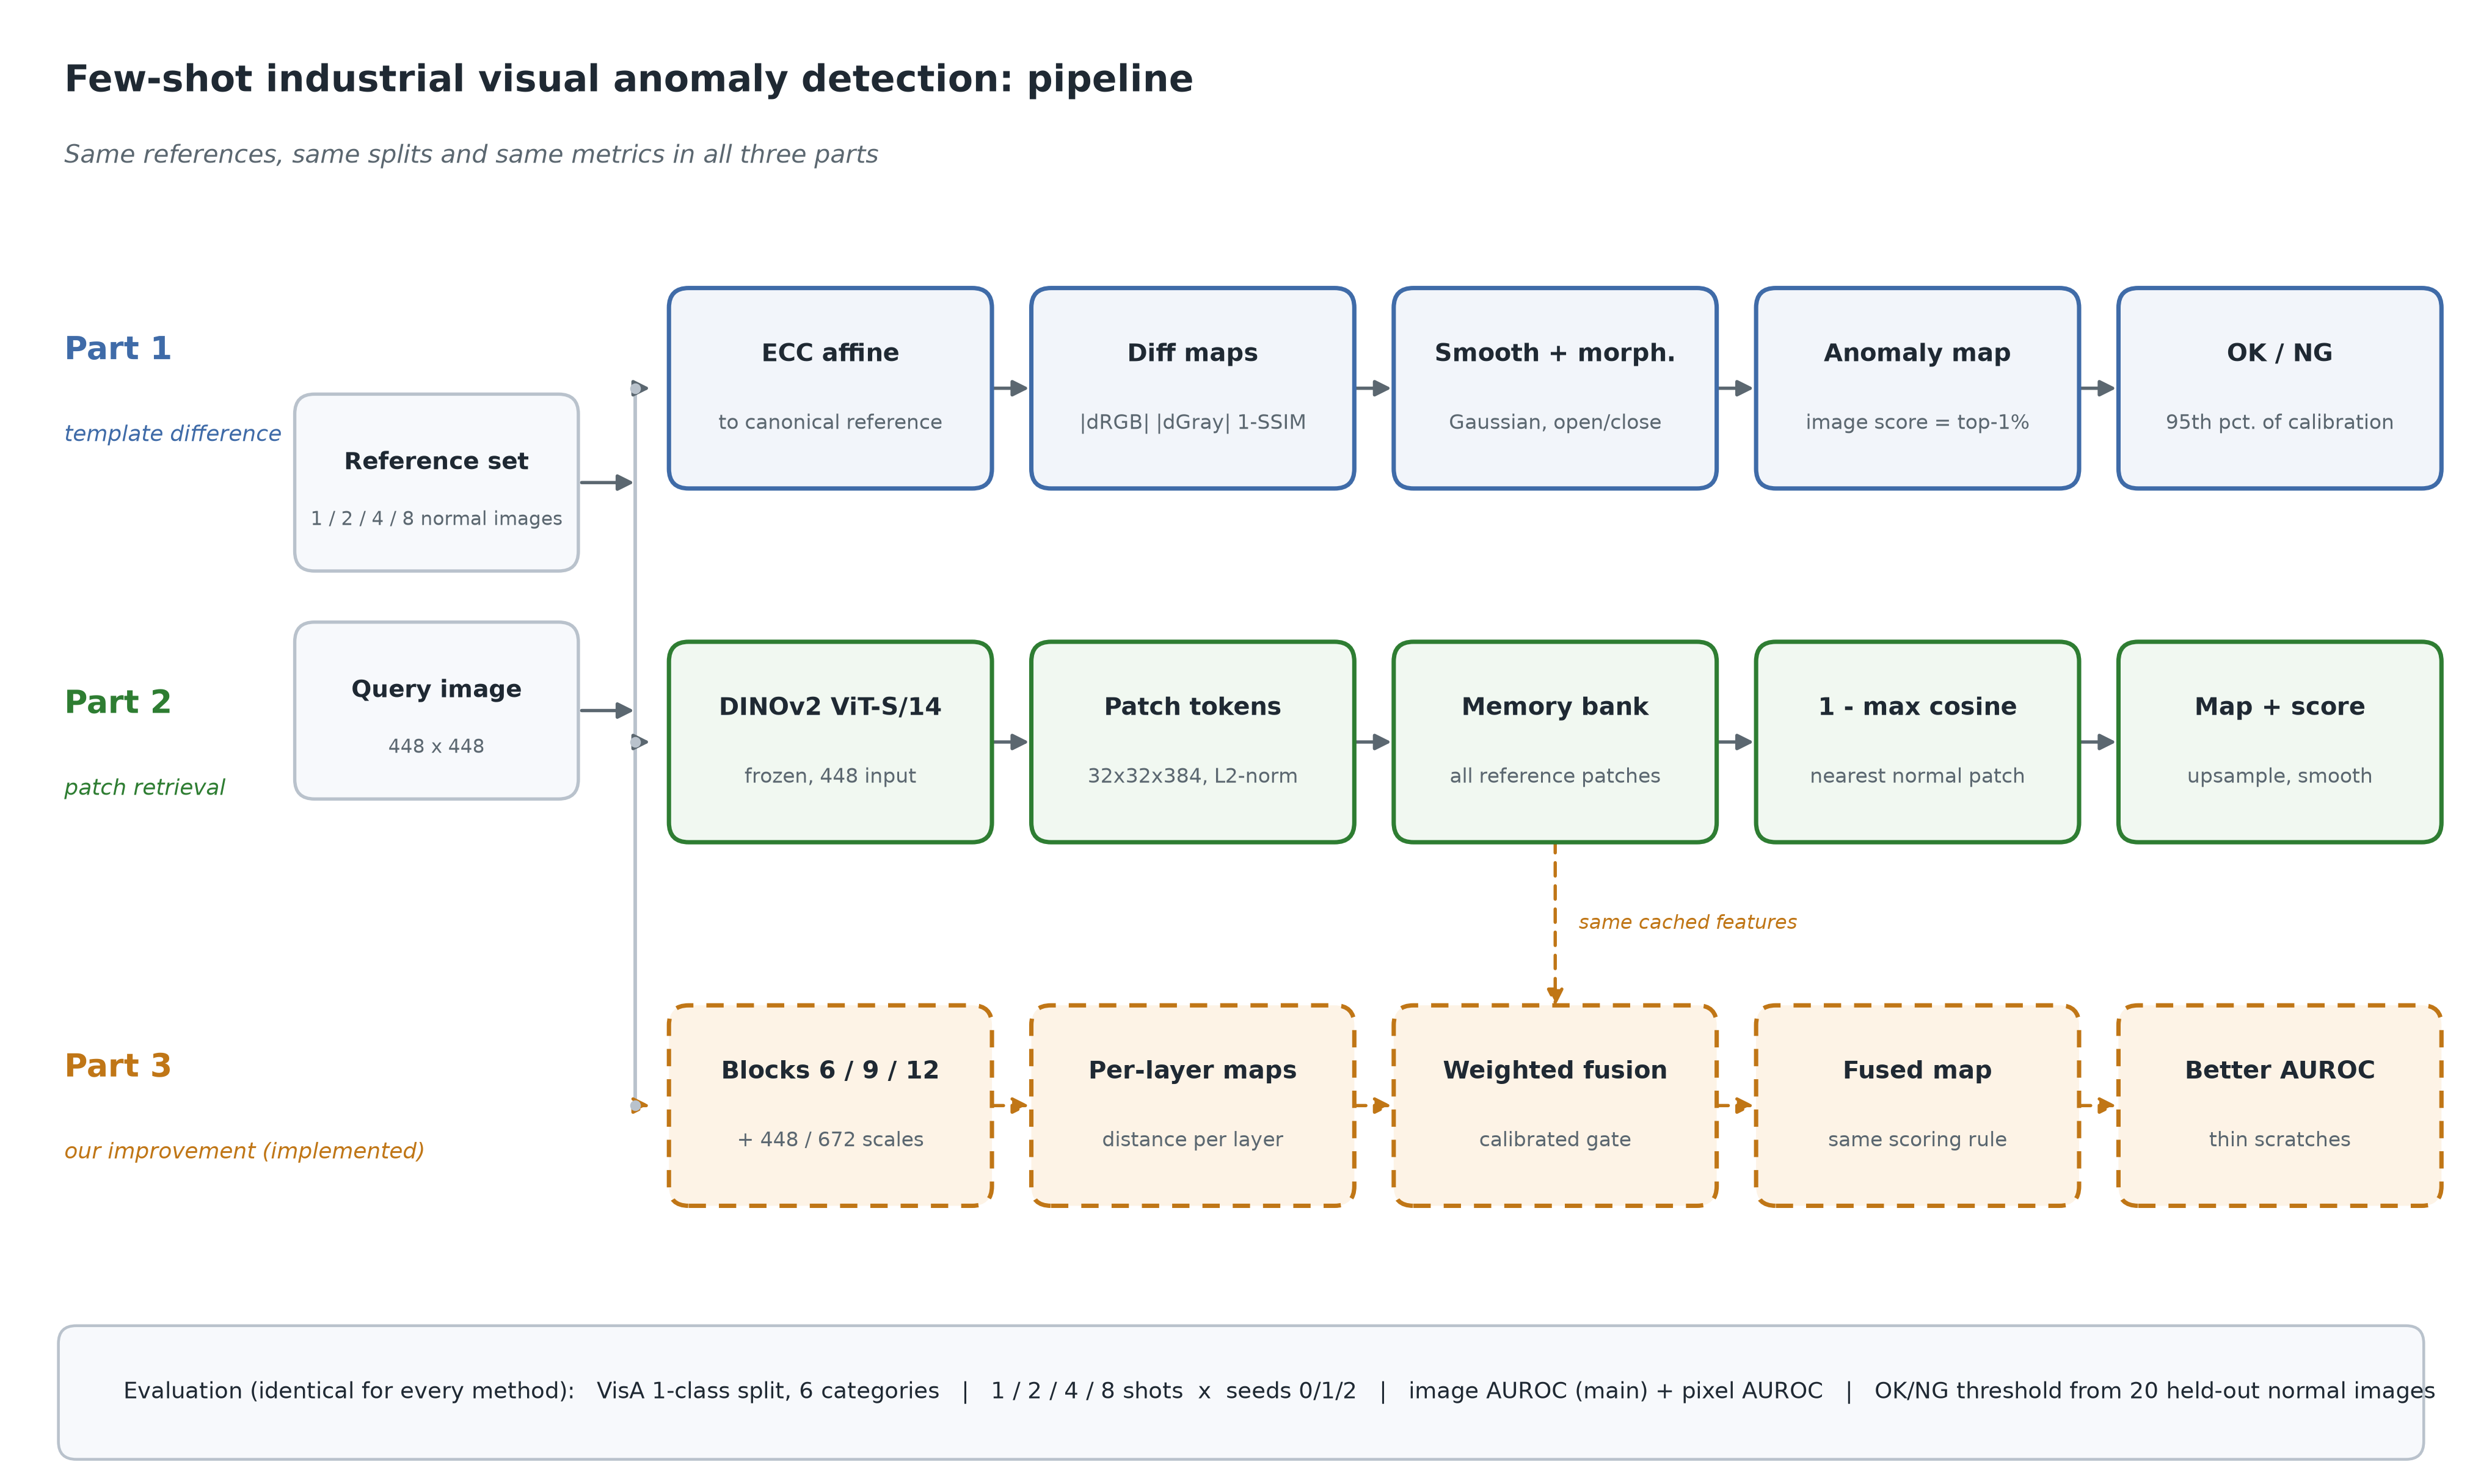
\includegraphics[width=0.95\linewidth]{figs/pipeline.png}
\end{center}
\caption{The three parts of the system. Part 1 compares an aligned test image
with the reference set through three pixel-wise difference channels. Part 2
scores each patch of a frozen DINOv2 feature map by its distance to the nearest
normal patch. Part 3 fuses distance maps of three transformer blocks at two
scales before scoring. All parts share the same references, the same six
categories and the same metric code.}
\label{fig:pipeline}
\end{figure*}

% ---------------------------------------------------------------------------
\section{Experiments}

\subsection{Implementation details}

Part 2 and Part 3 are implemented in PyTorch with the \texttt{transformers}
DINOv2 weights; Part 1 uses OpenCV and scikit-image. The main grid runs on the
MPS backend of an Apple M-series laptop, the official reproduction runs on a
single RTX 4090 rented for two hours. Every number below is regenerated from
the per-run JSON files by a single script, so tables, figures and text cannot
disagree.

\begin{table*}[t]
\centering
\small
\setlength{\tabcolsep}{9pt}
\begin{tabular}{lcccc}
\toprule
Configuration & 1-shot & 2-shot & 4-shot & 8-shot \\
\midrule
Part 1: template difference & 71.7$\pm$1.8 & 74.8$\pm$2.0 & 76.5$\pm$0.7 & 78.3$\pm$0.4 \\
Part 2: patch-NN, our implementation & 91.7$\pm$0.2 & 93.6$\pm$0.4 & 94.5$\pm$0.2 & 95.3$\pm$0.3 \\
Part 2: AnomalyDINO, official code & 92.8$\pm$1.4 & 94.3$\pm$1.7 & 95.7$\pm$0.9 & 96.6$\pm$0.2 \\
\midrule
Part 3: 448, block 12 (control) & 91.6$\pm$0.2 & 93.5$\pm$0.5 & 94.5$\pm$0.2 & 95.3$\pm$0.2 \\
Part 3: 448, blocks 6+9+12 & 94.2$\pm$0.4 & 95.3$\pm$0.2 & 95.8$\pm$0.1 & 96.1$\pm$0.3 \\
Part 3: 448+672, block 12 & 92.6$\pm$0.5 & 94.2$\pm$0.6 & 95.1$\pm$0.2 & 95.8$\pm$0.3 \\
Part 3: 448+672, blocks 6+9+12 & 94.4$\pm$0.6 & 95.6$\pm$0.3 & 96.3$\pm$0.1 & 96.4$\pm$0.2 \\
\bottomrule
\end{tabular}
\caption{Image-level AUROC (\%), six-category mean $\pm$ std over three reference selections.}
\label{tab:image}
\end{table*}
\begin{table*}[t]
\centering
\small
\setlength{\tabcolsep}{9pt}
\begin{tabular}{lcccc}
\toprule
Configuration & 1-shot & 2-shot & 4-shot & 8-shot \\
\midrule
Part 1: template difference & 72.9$\pm$0.3 & 73.4$\pm$0.5 & 73.7$\pm$0.3 & 74.0$\pm$0.3 \\
Part 2: patch-NN, our implementation & 96.5$\pm$0.5 & 97.3$\pm$0.2 & 97.8$\pm$0.1 & 98.0$\pm$0.1 \\
Part 2: AnomalyDINO, official code & 97.7$\pm$0.0 & 97.9$\pm$0.0 & 98.1$\pm$0.0 & 98.2$\pm$0.0 \\
\midrule
Part 3: 448, block 12 (control) & 96.5$\pm$0.6 & 97.2$\pm$0.2 & 97.8$\pm$0.1 & 97.9$\pm$0.1 \\
Part 3: 448, blocks 6+9+12 & 97.8$\pm$0.2 & 98.2$\pm$0.0 & 98.4$\pm$0.0 & 98.5$\pm$0.0 \\
Part 3: 448+672, block 12 & 97.3$\pm$0.5 & 97.9$\pm$0.1 & 98.3$\pm$0.0 & 98.4$\pm$0.1 \\
Part 3: 448+672, blocks 6+9+12 & 98.1$\pm$0.2 & 98.5$\pm$0.1 & 98.7$\pm$0.0 & 98.8$\pm$0.0 \\
\bottomrule
\end{tabular}
\caption{Pixel-level AUROC (\%), computed at $448\times448$ and averaged over the six categories.}
\label{tab:pixel}
\end{table*}

\subsection{Main results}

Tables~\ref{tab:image} and~\ref{tab:pixel} report image- and pixel-level AUROC
for all methods. Three observations stand out. First, the classical baseline
improves only from $71.7$ to $78.3$ as the number of references grows: its
ceiling is set by the representation, not by the amount of data. Second, a
frozen patch representation with a memory bank starts at $91.7$ with a single
reference, twenty points above the eight-shot baseline, and improves steadily
to $95.3$. Third, our fusion pushes the method to $94.4$ and $96.4$, which is
above the official implementation at one, two and four references and $0.2$
points below it at eight.

Table~\ref{tab:percat} breaks the four-shot result down by category. The
baseline is weakest exactly where the object layout changes between shots:
\emph{capsules} ($67.8$) and \emph{pipe fryum} ($70.4$), the two categories with
multiple or repositioned instances, while the well-aligned \emph{cashew} already
reaches $90.4$. Patch retrieval lifts every category above $92.5$ and the fused
model above $94$; the remaining weakness of the baseline is therefore a property
of the pixel-wise comparison, not of one hard category.

\begin{table}[t]
\centering
\small
\begin{tabular}{lccc}
\toprule
Category & Part 1 & Part 2 (ours) & Part 3 (fused) \\
\midrule
candle & 71.5 & 92.5 & 94.1 \\
capsules & 67.8 & 92.5 & 94.5 \\
cashew & 90.4 & 93.7 & 97.0 \\
chewinggum & 82.7 & 96.9 & 97.6 \\
fryum & 76.6 & 93.5 & 96.0 \\
pipe fryum & 70.4 & 97.8 & 98.4 \\
\bottomrule
\end{tabular}
\caption{Per-category image AUROC (\%) at 4-shot; mean over three seeds.}
\label{tab:percat}
\end{table}

\subsection{Ablation: which factor contributes what}

The eight configurations of Table~\ref{tab:image} form a $2\times 2$ factorial
design plus controls. Using blocks $6+9+12$ instead of block $12$ alone gives
$+2.6$ points at one-shot ($91.6\rightarrow94.2$) but only $+0.8$ at eight-shot;
adding the $672$ scale to a single block gives $+1.0$ and $+0.5$. The two axes
compose almost additively: the fused model is $+2.8$ above the single-block,
single-scale control at one-shot and $+1.1$ at eight-shot. The pattern is
consistent with the intuition that low-shot regimes lack evidence and therefore
benefit most from a richer descriptor, while with eight references the memory
bank already covers the normal variation. Pixel AUROC follows the same ordering
($96.5\rightarrow98.1$ at one-shot), which indicates that the gain is not an
artefact of the image-level aggregation.

\subsection{Where does the fusion help?}

Table~\ref{tab:gain} breaks the aggregate gain down by category. Fusion helps
five of the six categories at both shot counts, and the gain is largest exactly
where the control is weakest: \emph{cashew} improves by $9.2$ points at
one-shot ($86.3\rightarrow95.5$), \emph{capsules} by $4.3$, while categories
that the single-block model already handles well (\emph{chewinggum},
\emph{fryum}) move by less than two points. The single exception is
\emph{fryum} at one-shot ($-0.2$), which is well inside the $\pm0.6$ seed
spread of that configuration. At eight-shot every gain shrinks to between
$+0.4$ and $+2.2$, again consistent with the memory bank already covering the
normal variation when references are plentiful.
Figure~\ref{fig:p3qual} shows the effect on a single image: with three blocks
and two scales the response becomes broader along the crack of the \emph{fryum}
sample while the peak stays on the defect, and on \emph{chewinggum} the map
remains concentrated on the annotated spot.

\begin{table*}[t]
\centering
\small
\begin{tabular}{lcccccc}
\toprule
 & \multicolumn{3}{c}{1-shot} & \multicolumn{3}{c}{8-shot} \\
\cmidrule(lr){2-4}\cmidrule(lr){5-7}
Category & control & fused & $\Delta$ & control & fused & $\Delta$ \\
\midrule
candle & 91.0 & 93.1 & +2.1 & 93.4 & 94.9 & +1.5 \\
capsules & 87.6 & 92.0 & +4.3 & 92.8 & 94.5 & +1.6 \\
cashew & 86.3 & 95.5 & +9.2 & 96.6 & 97.5 & +1.0 \\
chewinggum & 94.8 & 96.6 & +1.8 & 97.1 & 97.6 & +0.5 \\
fryum & 93.8 & 93.6 & -0.2 & 95.0 & 97.2 & +2.2 \\
pipe fryum & 94.8 & 97.5 & +2.7 & 98.0 & 98.4 & +0.4 \\
\bottomrule
\end{tabular}
\caption{Per-category image AUROC (\%) of the fused model against the single-block, single-scale control (block 12 @448). Fusion helps five of six categories at 1-shot and all six at 8-shot; the gain is largest where the control is weakest (cashew) and shrinks as references grow.}
\label{tab:gain}
\end{table*}

\begin{figure}[t]
\begin{center}
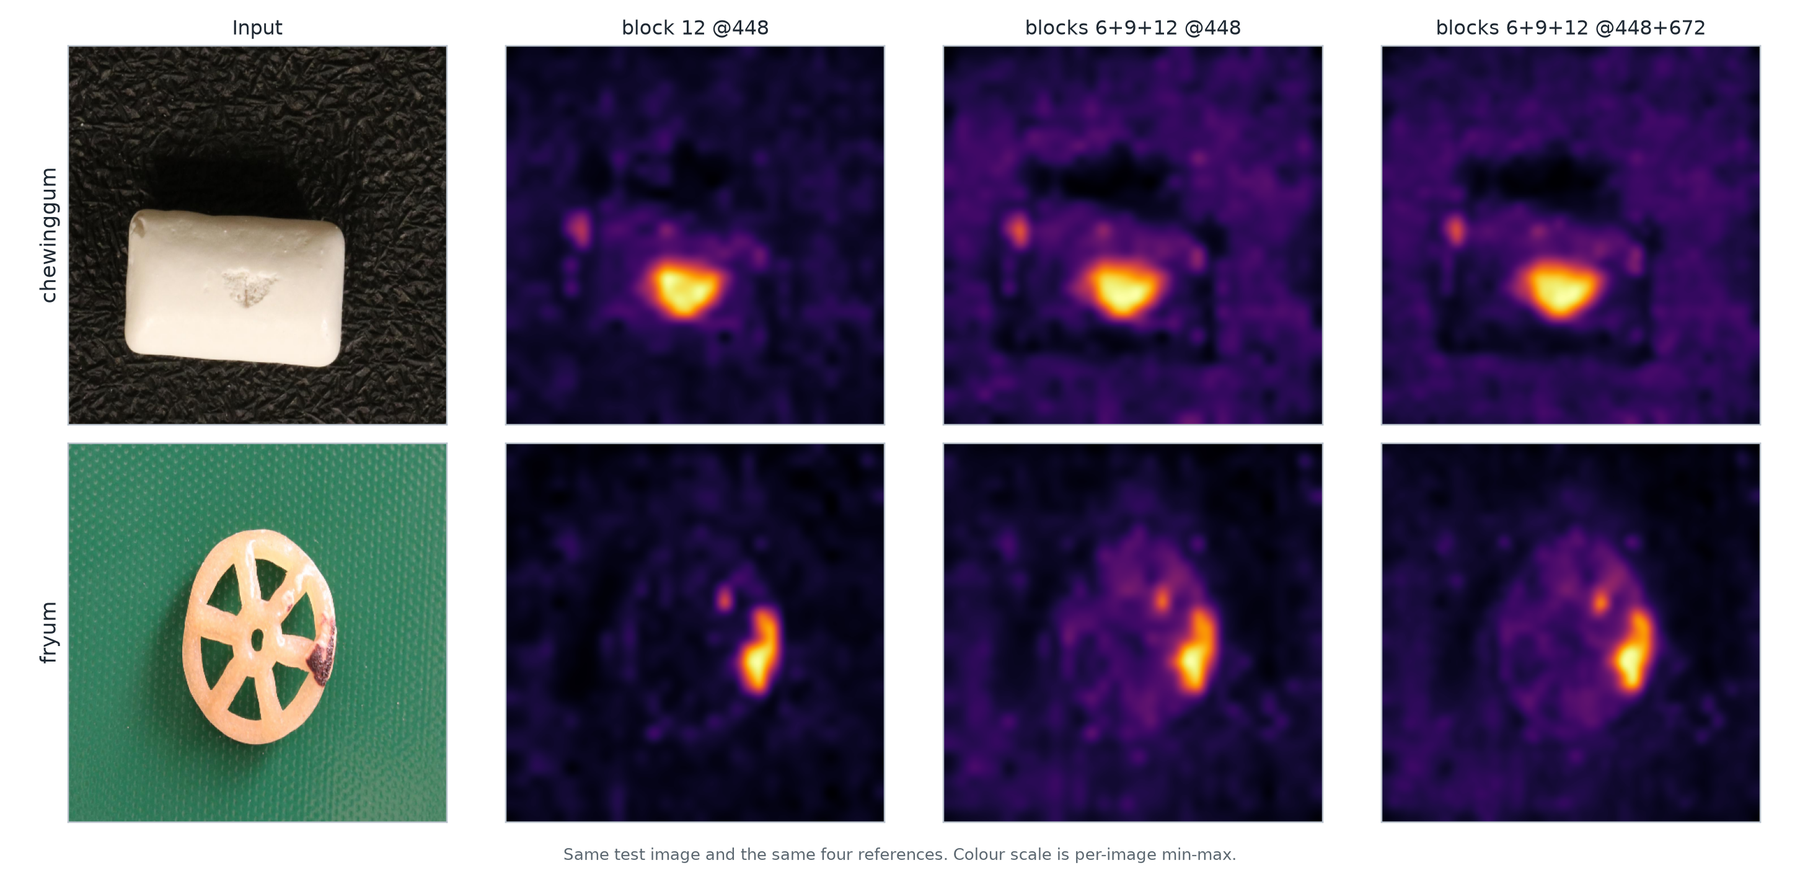
\includegraphics[width=\linewidth]{figs/part3_qual.png}
\end{center}
\caption{What the fusion changes visually (same image, same four references).
Block 12 alone already peaks on the defect; adding blocks $6+9$ and a $672$
scale widens the response along elongated defects and stabilises it on the
object, without introducing background peaks.}
\label{fig:p3qual}
\end{figure}

\subsection{Comparison with the official implementation}

The reproduced AnomalyDINO reaches $92.8/94.3/95.7/96.6$ image AUROC. Our
fusion reaches $94.4/95.6/96.3/96.4$ without PCA masking and without rotation
augmentation; at eight-shot the two are within $0.2$ points, i.e.\ inside the
seed-to-seed spread of the official run ($\pm0.2$). The per-category behaviour
explains why masking is not a free win: on the official run it lifts
\emph{capsules} from $89.8$ to $98.7$ but depresses \emph{candle} from $90.9$ to
$87.3$, because a foreground mask removes background patches that are, for this
category, part of the evidence. We therefore treat masking as a
\emph{when-to-apply} question rather than a fixed preprocessing step, and leave
it to future work.

The advantage of our fusion is concentrated in the low-shot regime, and the
reason is structural rather than a matter of tuning. With one reference image
the memory bank contains a single view of the object, so any descriptor that
happens to be weak for that view limits the whole system; averaging distance
maps from three blocks and two scales behaves like a small ensemble of
descriptors, which is exactly what a single reference cannot provide. As
references grow the bank covers more of the normal variation and the ensemble
effect saturates, which is why the gap narrows to $0.2$ points at eight-shot.
This also means the improvement costs nothing at test time: all distance maps
are computed from features that were already extracted, and the additional
arithmetic is a sum over at most six arrays of size $448\times448$.

\subsection{Qualitative results}

Figure~\ref{fig:comparison} shows the same two test images under the baseline
and under patch retrieval, together with the ground-truth mask. On
\emph{chewinggum} the baseline responds to the outline of the object, a
misalignment artefact, while the patch map peaks on the defect; on
\emph{candle} the baseline lights up the rim of every candle in the frame and
the patch map selects the missing piece. Figure~\ref{fig:curves} summarises the
shot dependence of every configuration.

\begin{figure*}[t]
\begin{center}
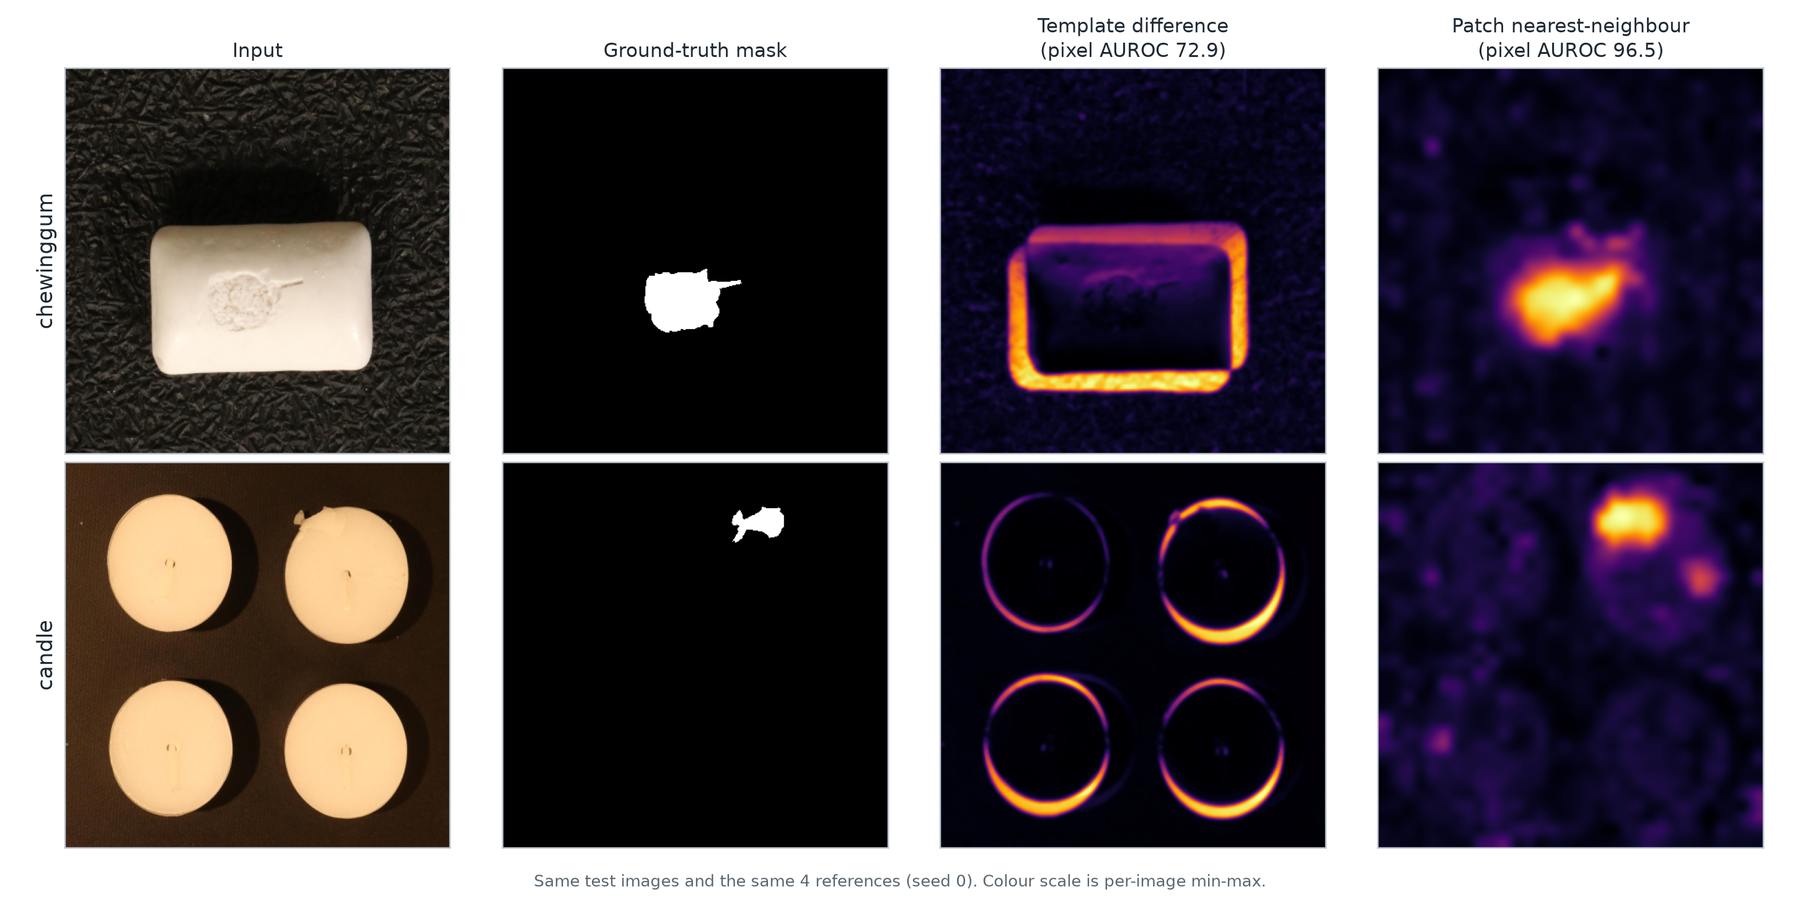
\includegraphics[width=0.92\linewidth]{figs/comparison.png}
\end{center}
\caption{Qualitative comparison with the same four references. Left: the
classical baseline highlights object outlines; right: patch retrieval localises
the defect. Colour scales are per-image min-max.}
\label{fig:comparison}
\end{figure*}

\begin{figure*}[t]
\begin{center}
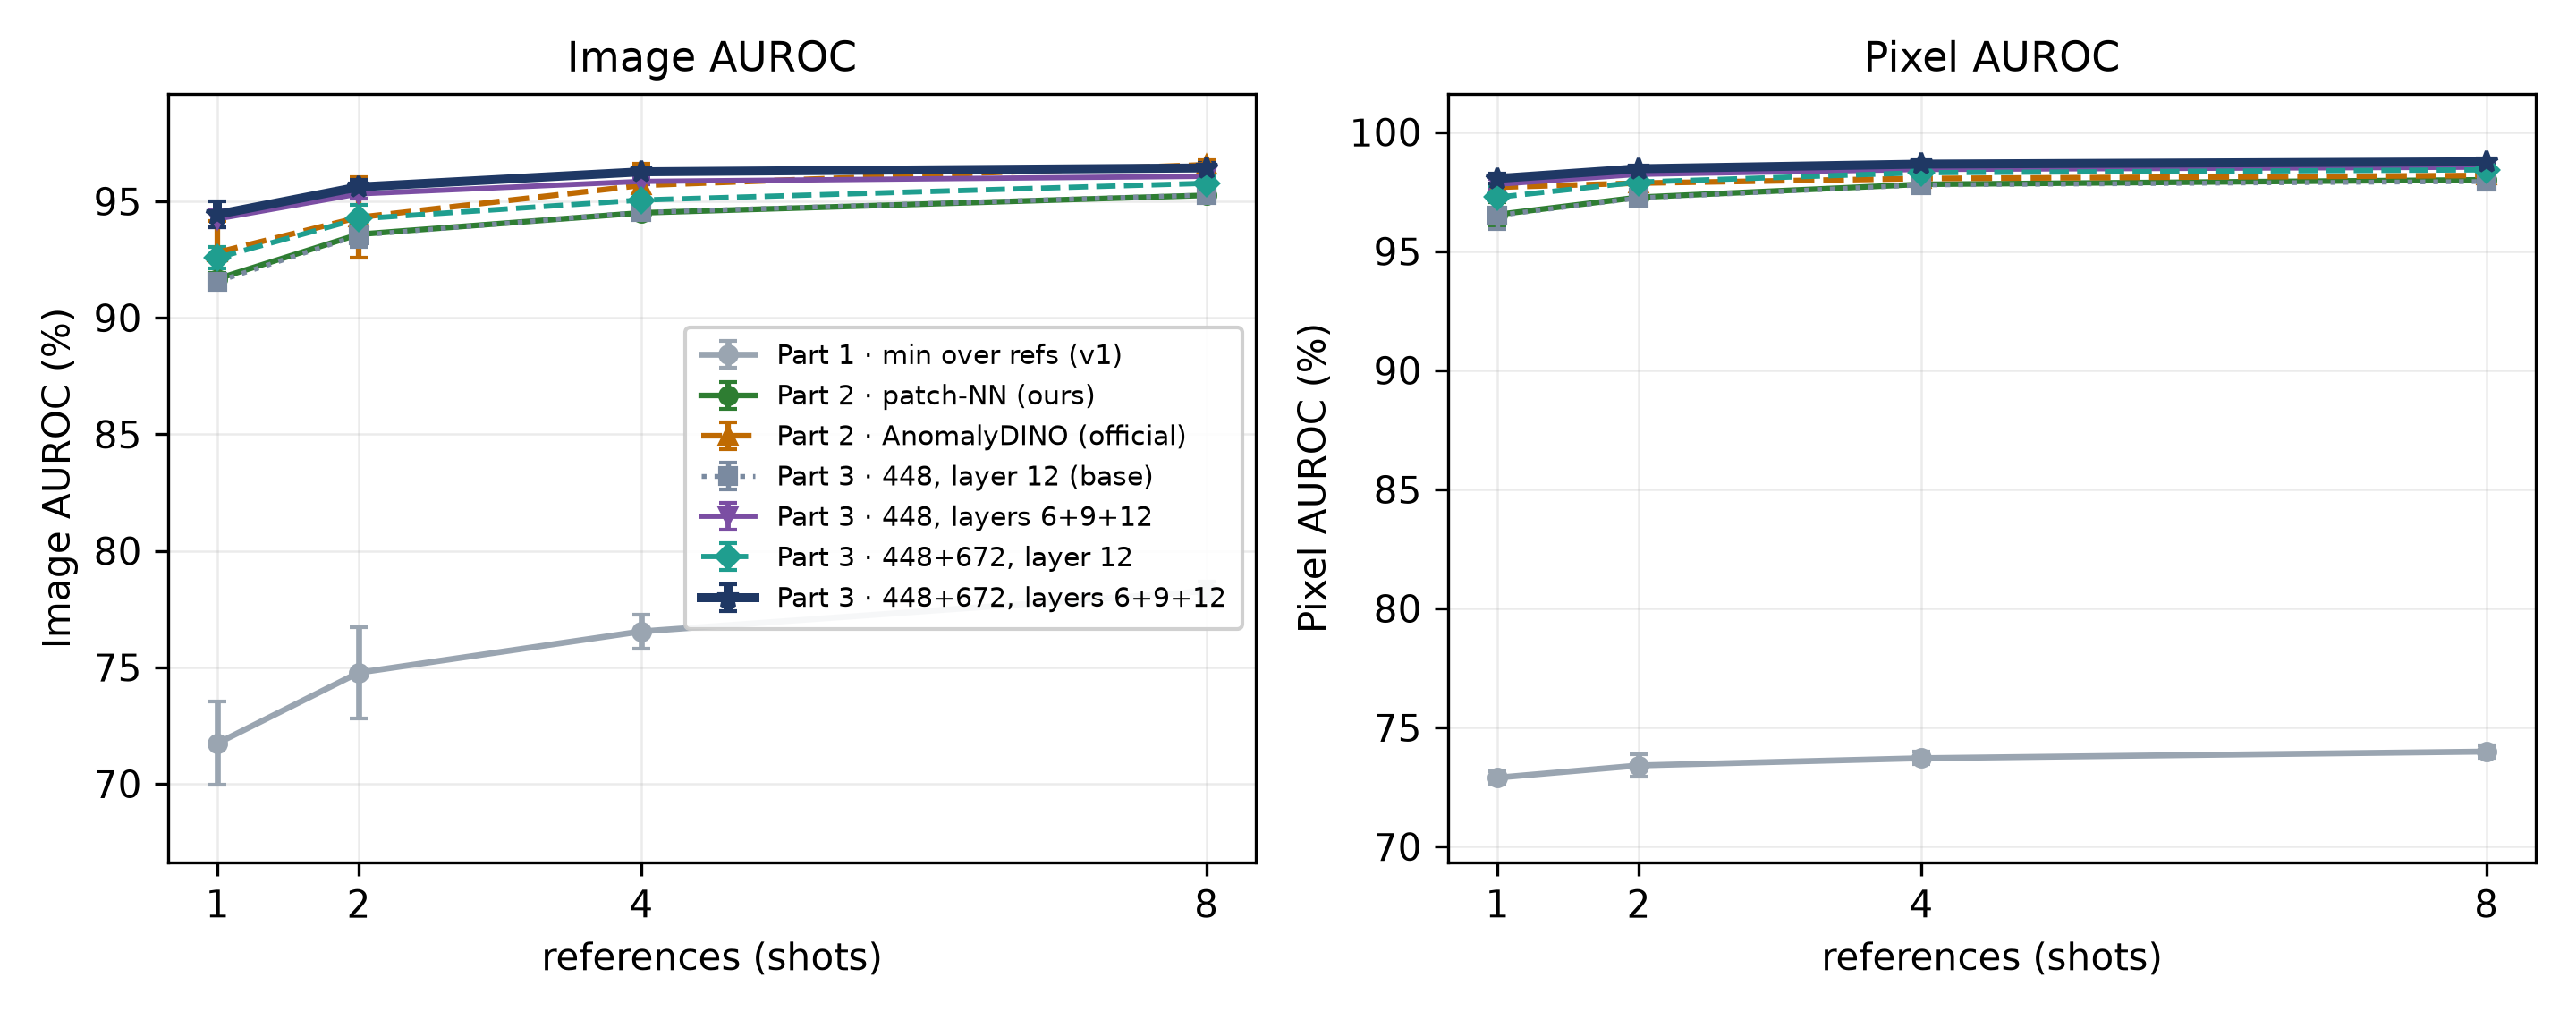
\includegraphics[width=0.95\linewidth]{figs/auroc_vs_shot.png}
\end{center}
\caption{Image- and pixel-level AUROC as a function of the number of references.
The multi-layer, multi-scale fused model dominates at every shot count, and the
gap to the baseline does not close with more references.}
\label{fig:curves}
\end{figure*}

\subsection{Why does the pixel-wise baseline fail?}
\label{sec:failure}

On \emph{chewinggum} the baseline reaches a pixel AUROC of $0.40$, i.e.\ below
chance, while patch retrieval reaches $0.97$ on exactly the same masks. The
median defect on this category covers $0.53\%$ of the image
(Table~\ref{tab:dataset}), i.e.\ about one part in two hundred. We
checked that this is not an artefact of the annotations: the masks are the same
objects that the patch method localises almost perfectly. We then measured, for
six anomalous test images, the mean residual inside and outside the ground-truth
mask: $0.21$--$0.27$ inside versus $0.22$--$0.23$ outside, with ratios between
$0.90$ and $1.16$. The map therefore carries essentially no localisation signal
for this category. Part of the constant $\approx0.22$ offset comes from our
global $1-\mathrm{SSIM}$ term; removing it leaves the spatial part still weak
(pixel AUROC $0.449$ on this category in a single-reference test), and replacing
it with a local SSIM map made localisation worse ($0.288$), because the textured
background dominates. Two further controls rule out the obvious alternatives:
per-reference re-alignment changes pixel AUROC only from $38.9$ to $39.4$, and
the ECC warp is demonstrably effective (mean grey residual on this category
drops from $0.121$ to $0.046$, a $62\%$ reduction, with correlation coefficient
$0.986$). The failure is a property of the representation: a pixel-wise residual
measures how similar two photographs are overall, and a defect that occupies
about $1\%$ of the pixels is invisible next to a global appearance offset.

\textbf{Threats to validity.} Three choices bound what our numbers can claim.
First, the six categories were fixed by the brief, so nothing here says how the
fusion behaves on the four PCB categories of VisA, which are structurally
harder. Second, our pixel AUROC is computed at the prediction resolution
($448\times448$) rather than at the native mask resolution, which flatters
methods with coarse maps; since every method is measured the same way the
ranking is unaffected, but the absolute values are not comparable to papers that
evaluate at native resolution. Third, three reference selections per shot give
standard deviations of one to two points, so differences smaller than that
should be read as ties --- which is the case for our fused model against the
official implementation at eight-shot.

\begin{table*}[t]
\centering
\small
\begin{tabular}{llcc}
\toprule
Stage & Device & Per image & Peak memory \\
\midrule
Part 1 template difference, 4 refs (incl.\ ECC) & Apple M-series CPU & 57.7\,ms & 2.0\,GB RSS \\
Part 2 feature extraction, ViT-S/14 @448 & Apple M-series MPS & 37\,ms & 2.0\,GB unified \\
Part 2 retrieval, 1 reference & Apple M-series MPS & 0.8\,ms & -- \\
Part 2 retrieval, 8 references & Apple M-series MPS & 3.2\,ms & -- \\
Official AnomalyDINO inference & RTX 4090 24\,GB & 46\,ms & 0.6\,GB observed \\
\bottomrule
\end{tabular}
\caption{Runtime and memory per image, on the device each experiment was run. Feature extraction is cached once (4,205 images, $\approx$4 min) and is excluded from the retrieval rows.}
\label{tab:efficiency}
\end{table*}

\subsection{Efficiency}

Table~\ref{tab:efficiency} reports runtime and memory on the device each
experiment was run, as required for a fair comparison. The baseline costs
$57.7$\,ms per image on CPU; DINOv2 feature extraction costs $37$\,ms per image
on the laptop GPU and is paid once for the whole dataset; retrieval costs
$0.8$\,ms with one reference and $3.2$\,ms with eight. The complete $381$-run
grid therefore fits on a laptop, and the rented GPU was used only to run the
official code, whose environment (PyTorch, torchvision, FAISS) was the actual
reason for renting it rather than the compute. Peak memory is reported as the
process peak on unified memory for the Apple runs and as the device memory
observed with \texttt{nvidia-smi} for the $4090$ run.

% ---------------------------------------------------------------------------
\section{Conclusion}

We compared three levels of solution for few-shot defect-free inspection under
one protocol. The classical baseline saturates early and, on one category, fails
at the pixel level for a reason we can measure: its residual is numerically
identical inside and outside the defect. A frozen patch representation with a
memory bank is twenty points stronger with a single reference, and our
training-free fusion of three transformer blocks and two input scales adds a
further $2.8$ points at one-shot, reaching parity with the official
implementation at eight references and exceeding it at one to four.

\textbf{Limitations.} Our implementation omits the two preprocessing steps of
the official method (PCA masking, rotation augmentation), uses a square resize
and no ImageNet normalisation, and evaluates pixel AUROC at the prediction
resolution rather than at the native mask resolution. The official run samples
its references with its own random number generator, so the two implementations
share seeds and calibration rules but not necessarily the exact reference files.
Only six of the twelve VisA categories are used.

\textbf{Future work.} Three directions follow directly. First, decide
\emph{when} to apply background masking, using the per-category evidence above
and a foreground mask from Segment Anything \cite{kirillov2023sam}. Second,
calibrate the decision: the fixed $95$th-percentile threshold produces about
$10\%$ false positives and $55\%$ false negatives on the test split, so a
risk--coverage analysis and a selective ``uncertain'' output are the natural
next step. Third, evaluate pixel metrics at native resolution and with
\texttt{float16} retrieval to quantify the accuracy--cost trade-off of the
memory bank, following EfficientAD \cite{batzner2024efficientad}.

{\small
\bibliographystyle{ieeenat_fullname}
\bibliography{references}
}

\end{document}
